\title{$k$-Nearest Neighbors}
\label{chp:k-nearest-neighbors}
\author{George G. Cabral}
\institute{Department of Computing, Federal Rural University of Pernambuco, BR}




\maketitle

%\section{Introduction}

Among all supervised classifiers, the family of nearest neighbor (NN) based classifiers are, perhaps, the simplest and most intuitive ones. In a nutshell, given a set of examples $\mathcal{T}$ containing $n$ examples, and considering that we want to find the class of an unlabelled example \textbf{z}, the most basic form of NN (i.e., 1NN) finds the closest example (\textbf{x}$^{(i)}$) to \textbf{z}, among all $n$ examples in $\mathcal{T}$, and assigns the same class of \textbf{x}$
^{(i)}$ (i.e., $y^{(i)}$) to \textbf{z}.

In order to obtain the closest example, first it's necessary to define a distance, or a similarity, function. The Euclidean distance (Eq. \ref{eq:euclid_dist}) stands as the most widely used function. This metric consists in the distance between two examples in an $n$-dimensional Euclidean space. In Eq. \ref{eq:euclid_dist}, the distance between the examples \textbf{x}$^{(i)}$ and \textbf{z}, located in the $j_{th}$ dimensional space, is being computed.

\vspace{0.2cm}

\begin{equation}
    EuclidDist(\textbf{x}^{(i)},\textbf{z}) = \sqrt{(x^{(i)}_{1} - z_1)^{2} + (x^{(i)}_{2} - z_2)^{2} + \cdots + (x^{(i)}_j - z_j)^{2}}
    \label{eq:euclid_dist}
\end{equation}

\vspace{0.2cm}

In Figure \ref{fig:EucDistance}, the norm of the orange line (i.e., the length/distance between hypothetical examples \textbf{x} = [1,1] and \textbf{z} = [5,4]), obtained by using Eq. \ref{eq:euclid_dist}, is $\sqrt{(1-5)^2 + (1-4)^2}$ resulting in 5 units. 

\begin{figure}[h]
    \centering
    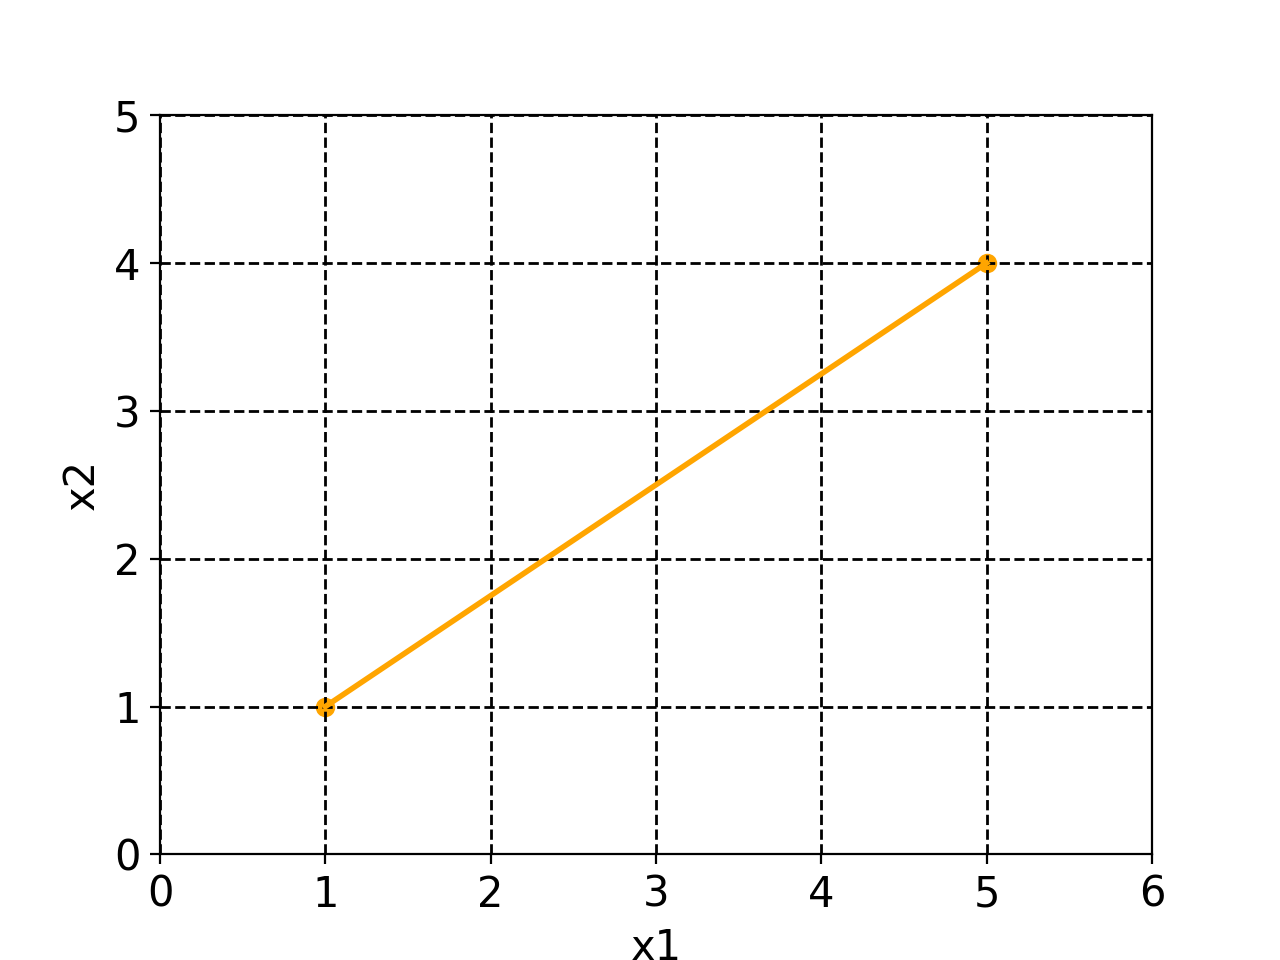
\includegraphics[height = 4.5cm, width =  5cm]{"Part 3 - Learning Systems/Supervised Learning/k-Nearest Neighbors/figures/EuclideanDistance2.png"}
    \caption{Euclidean Distance illustration between examples located at coordinates (1, 1) and (5, 4).}
    \label{fig:EucDistance}    
\end{figure}

Nevertheless, depending on the domain of the problem, the use of different distance functions might be more adequate. However, these functions must respect the following conditions:

\begin{itemize}
    \item Non-negativity: $d(x, y) \geq 0$
    \item Identity: $d(x, y) = 0$ if and only if $x = y$
    \item Symmetry: $d(x, y) = d(y, x)$    
    \item Triangle Inequality: $d(x, y) + d(y, z) >= d(x, z)$
\end{itemize} %fonte: https://www.kdnuggets.com/2020/11/most-popular-distance-metrics-knn.html

\section{Other Distance Metrics}

A number of different distances can be used according the domain of the specific application. Some of them are presented in the sequel:  

\subsection{Manhattan Distance}


The Manhattan distance \cite{Craw2010} (also known as taxicab or cityblock distance) between two examples in $j$-dimensional space is defined by the sum of the distances in each dimension. Equation \ref{eq:manDistance} computes this distance between two examples in the $j$-dimensional space.

\begin{equation}
    ManhDist(x,z) = \sum_{i=1}^{j} \|x_{i} - z_{i}\| 
    \label{eq:manDistance}
\end{equation}


Figure \ref{fig:manDistance} shows an example with two unit squares centered at coordinates (1.5, 1.5) and (4.5, 3.5). For this example, the Manhattan distance is $\|1.5 - 4.5\| + \|1.5 - 3.5\|$ resulting in 5 units.
 
\begin{figure}[h]
    \centering
    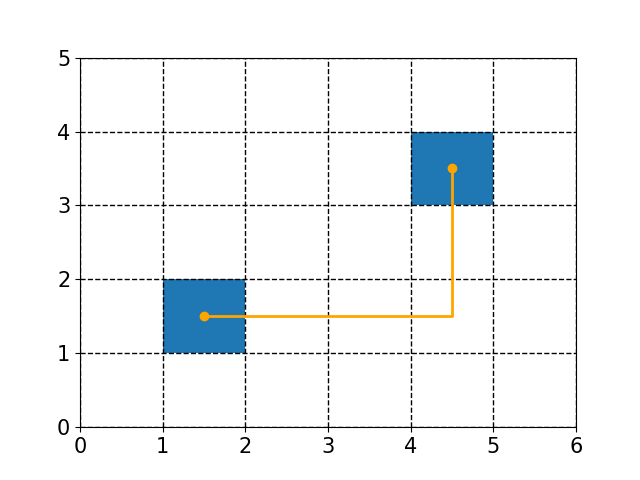
\includegraphics[height = 5cm, width =  5.5cm]{"Part 3 - Learning Systems/Supervised Learning/k-Nearest Neighbors/figures/manhattanDistance.png"}
    \caption{Manhattan Distance illustration between examples defined by coordinates (1.5, 1.5) and (4.5, 3.5).}
    \label{fig:manDistance}
\end{figure}

\subsection{Cosine Similarity}

The metric cosine similarity \cite{han2012mining} measures the angle between two vectors in the $j$-dimensional space. The intuition is that the smaller the angle between the two vectors is, more similar they are to each other.

This metric assumes the value 1 when two vectors are identical and the value -1 when they are completely opposite to each other. These situations take place when the angle between two vectors are 0 and 180 degrees (i.e., the vectors are parallel and have the same direction and the vectors are parallel but have opposite directions, respectively).

Equation \ref{eq:cosineSim} computes the cosine similarity. In Eq. \ref{eq:cosineSim}, assuming that \textbf{x} and \textbf{z} are both vectors, \textbf{x} $\cdot$ \textbf{z} = \textbf{x}$^t \cdot$ \textbf{z} and $\|$\textbf{x}$\| = \sqrt{x_1 \times x_2 \quad \cdots \quad x_n}$.

\begin{equation}
    CosSim(x,z) = \frac{x \cdot z}{\|x\| \times \|z\|}
    \label{eq:cosineSim}
\end{equation}

Among the applications of the cosine similarity is the documents similarity test. Documents can be represented by term-frequency vectors, i.e., each vector position contains the number of occurrences of a given term. 
%referencia Jiawei Han, ... Jian Pei, in Data Mining (Third Edition), 2012


\subsection{Hamming Distance}

The Hamming distance \cite{hamming:12} measures the number of characters in disagreement between two words, or two vectors, in general. In other words, the hamming distance is the number of symbols we must change in order to make a vector turn into another. Example: the Hamming distance between the words ``\textbf{de}ploys" and ``\textbf{em}ploys" is two. Notice that this distance requires the two words have the same length. 

The Hamming distance can be viewed as a special case of the Levenshtein distance where the words must have the same length. In contrast to Hamming Distance, the Levenshtein distance computes the number of substitutions, insertions or deletions necessary to turn one word into another.


\section{The kNN Algorithm Explained}

In contrast to other common machine learning families of algorithms, such as Neural Networks and Decision Trees, the $k$NN family of algorithms do not possess a learning phase yielding an abstract model representing the problem, instead, these algorithms only store the training examples. Given this fact, $k$NN like algorithms are also known as lazy algorithms. In the test phase, once a new unlabelled example \textbf{z} arrives: (i) its distances (or similarities) to all training examples are computed; (ii) the training examples are sorted accordingly to their distances to \textbf{z}; (iii) the most frequent class among the classes of the $k$ \textbf{z}'s nearest neighbors is then returned (note that for regression problems, the average of the target values from the $k$ \textbf{z}'s nearest neighbors is returned). 

Algorithm \ref{alg:knn} depicts the test procedure for the original $k$NN . In Alg. \ref{alg:knn}, $\mathcal{T}$ is a set of training examples consisting of tuples (\textbf{x},$y$), \textbf{z} is an unlabelled test example and $k$ is the number of neighbors to be considered. In line 1, $neighbors$ is an empty list that shall store tuples containing a distance $d$ (between a training example \textbf{x}$^{(i)}$ and a test example \textbf{z}) and the label $y^{(i)}$. The loop from lines 2 to 4 fills the $neighbors$ list and in line 6 this list is sorted in ascending order according the stored distances $d$. The returned class label ($y^{'}$) will be the most frequent class considering the first $k$ items of $neighbors$ (or the average of the \textit{k} \textbf{z}'s neighbors target values for regression problems, as aforementioned).

\vspace{0.2cm}

\begin{algorithm}[ht!]
    \caption{Simple $k$ Nearest Neighbor}
    
    Parameters: $\mathcal{T}$,$z$,$k$
    
    Output: $y^{'}$
    
    \begin{algorithmic}[1] 
    
    \STATE $neighbors \gets []$
    
    \FOR{$\mathbf{x}^{(i)} \in \mathcal{T}$}
    
      \STATE $d$ $\gets$ distance($\mathbf{x}^{(i)}$,$z$)
    
      
      \STATE $neighbors[i]$ $\gets$ ($d$,$y^{(i)}$)
    
    \ENDFOR
    
    
    \STATE sort(neighbors)
    
    
    \STATE $y^{'}$ $\gets$ mode($neighbors[0:k]$)
    
    
    \end{algorithmic}


\label{alg:knn}
    
\end{algorithm}


\vspace{0.2cm}

For the 1NN ($k = 1$), the Voronoi space for a set of two dimensional examples depicts the boundaries of the areas covered by each training example. Figure \ref{fig:voronoi} presents a Voronoi space defined by the depicted blue examples. In this Figure, dashed lines represent infinite boundaries. Since each region is defined by a training example, a new unlabelled example will receive the label of the example that defined the region. By way of illustration, given that the example \textbf{p} defines the class of the orange region, the same class of \textbf{p} will be assigned to all unlabelled examples placed in this region.


\begin{figure}[h]
    \centering
    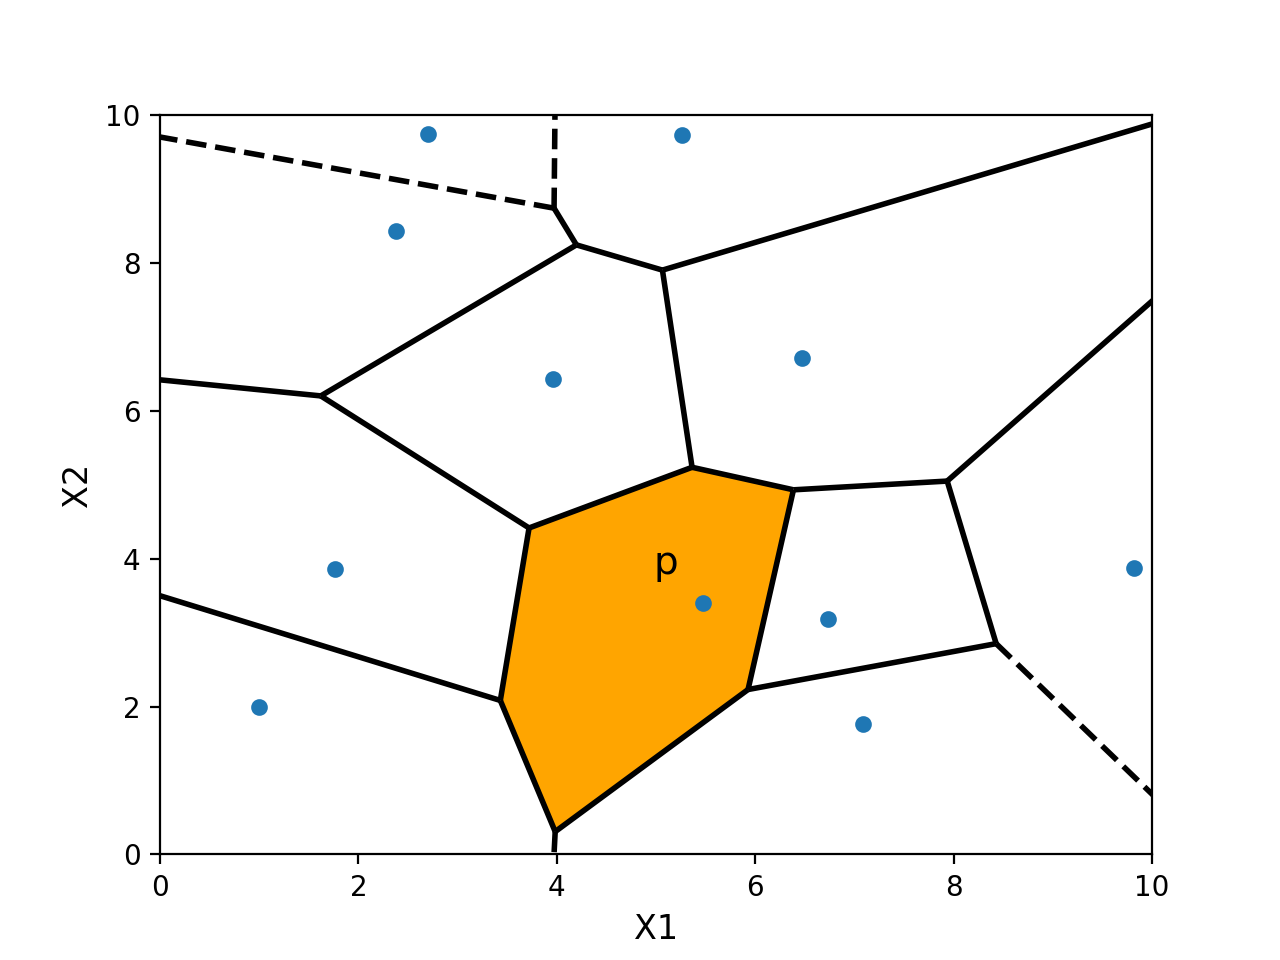
\includegraphics[height = 7cm, width =  8.5cm]{"Part 3 - Learning Systems/Supervised Learning/k-Nearest Neighbors/figures/voronoi2.png"}
    \caption{Voronoi space delimiting the 1NN decision boundaries. Dashed lines represent boundaries of infinite length.}
    \label{fig:voronoi}
\end{figure}

Figure \ref{fig:decisionboundaries} presents the different decision regions generated by the $k$NN using different $k$ values applied to a two overlapping classes dataset (blue and orange examples). Firstly, it is important to notice that some examples close to the center of the plot seems to be placed in conflicted regions. These examples, according to the domain of the problem, may be considered noisy or not. Nevertheless, when using $k = 1$ (Figure \ref{fig:decisionboundaries}.a)), potential noisy examples will have the same importance in building the decision boundaries as any other example (i.e., when $k = 1$ the $k$NN is completely adjusted to the examples in the training set resulting in an \textbf{overfitting} of the data). In Figure \ref{fig:decisionboundaries}.b) a $k = 3$ was used and the effect of an isolated orange example (placed inside the distribution of blue examples) in the decision process was largely reduced. Also, it is noticeable that in Figures \ref{fig:decisionboundaries} c) and d) the decision surface becomes smoother and the importance of noisy examples tends to disappear; as expected for larger values of \textit{k}. 

\begin{figure}[h]
    \centering
    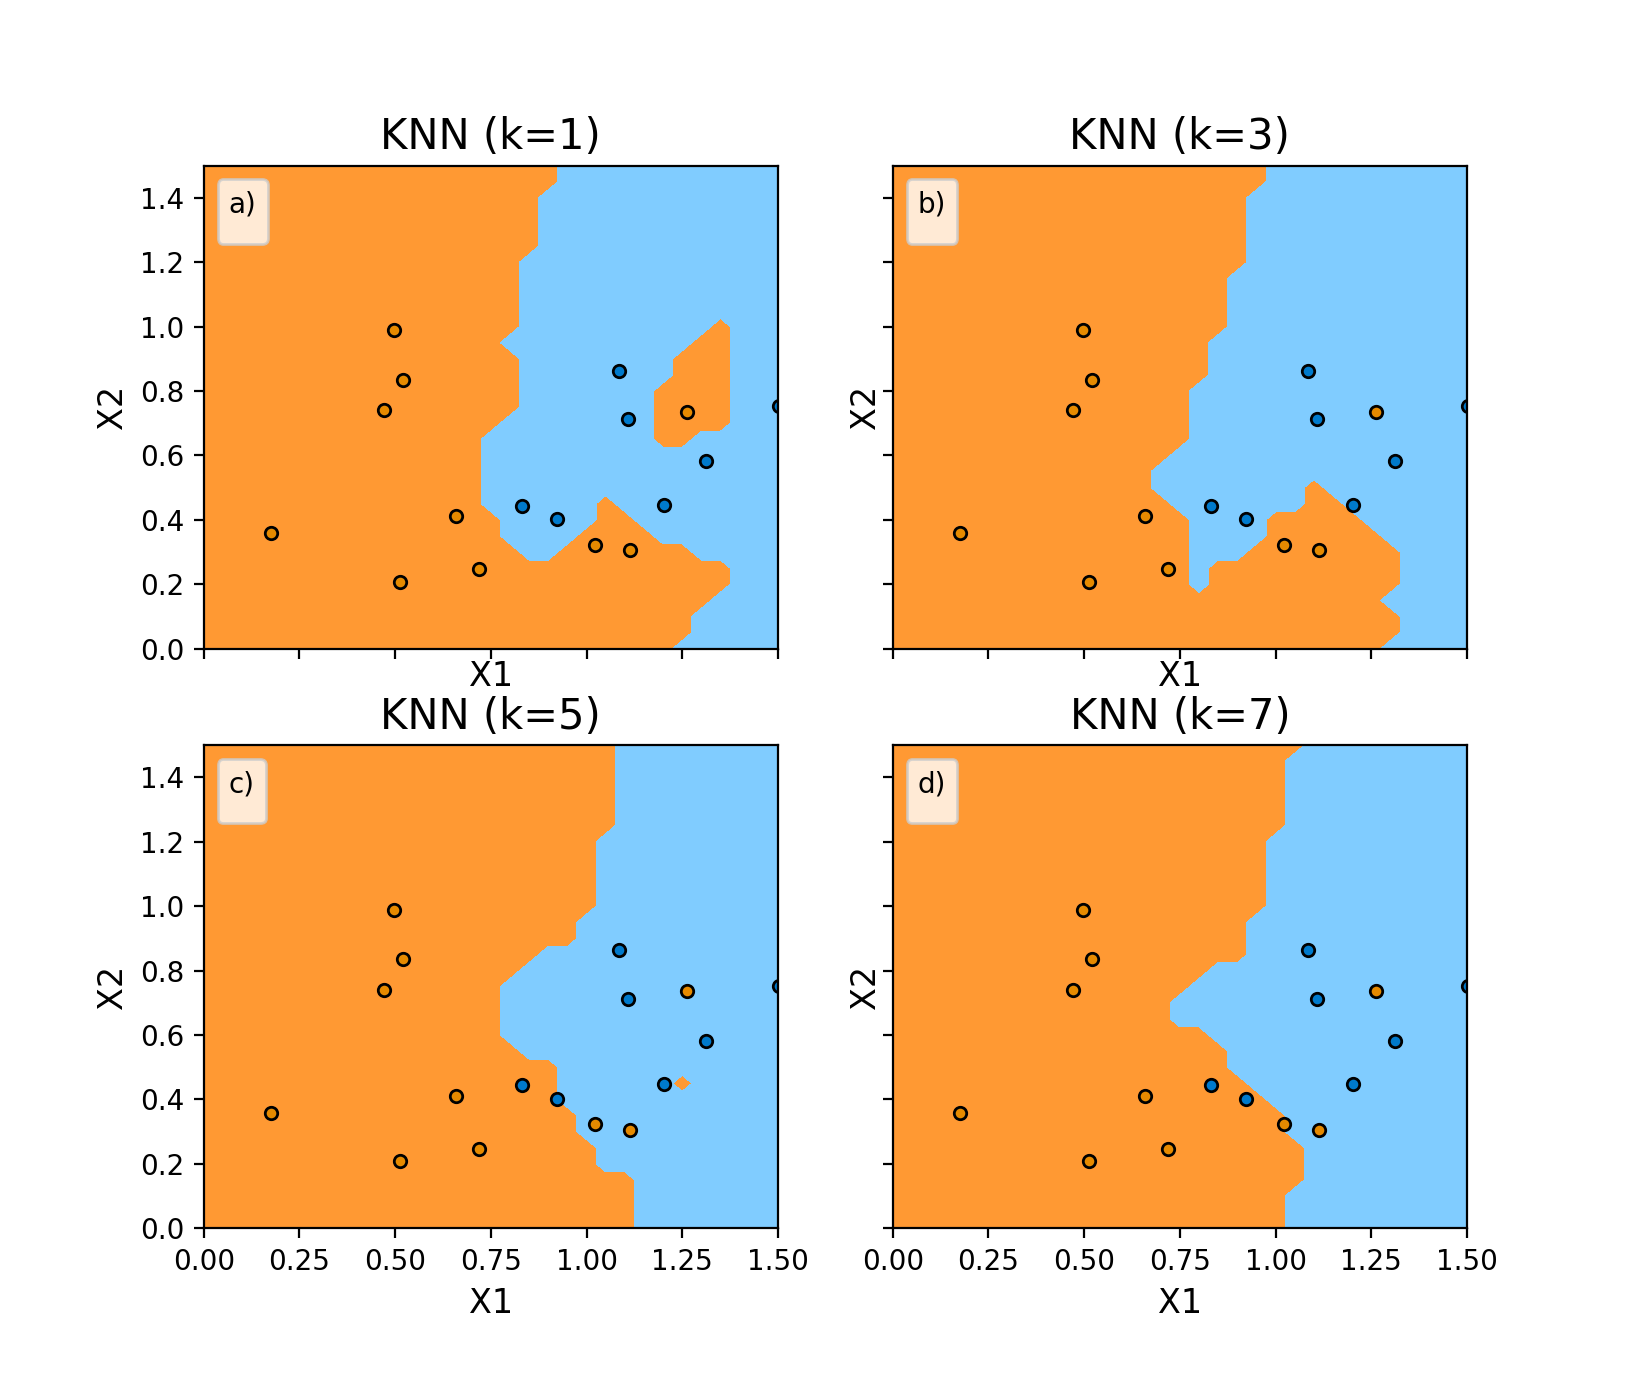
\includegraphics[height = 11cm, width =  14cm]{"Part 3 - Learning Systems/Supervised Learning/k-Nearest Neighbors/figures/decision_boundaries2.png"}
    \caption{Decision boundaries for different $k$ odd values ranging from 1 to 7.}
    \label{fig:decisionboundaries}
\end{figure}

\section{Prototype Reduction Schemes}

As aforementioned, the training phase of original the $k$NN consists solely of storing the training examples. On the other hand, the test phase, as shown in Alg. \ref{alg:knn}, requires the computation of the distance among each training example and the test example to be classified. In addition, it requires the usage of a sorting algorithm. These two tasks may lead to an unacceptable computational burden in the case of an exceedingly large training set. 

With the aim of reducing the computational cost at the test phase, Prototype Reduction Schemes (PRSs) have been used to reduce the size of the training set while keeping, or causing an acceptable loss, in the predictive performance. In sequel, two simple and popular PRSs will be presented: Condensed Nearest Neighbor (CNN) \cite{cnn:68} and Nearest Neighbor with Structural Risk Minimization (NNSRM) \cite{nnsrm:2003}.

\subsection{Condensed Nearest Neighbor - CNN}

The Condensed Nearest Neighbor was initially proposed by P. Hart \cite{cnn:68}. The basic intuition behind CNN is to scan all training examples in order to find the incorrectly classified ones according to the 1NN and to store them in an array $S$. By doing this, the method is capable of discarding redundant information and, as consequence, keeping only the most representative examples of the problem, i.e., the examples placed in conflict areas. 


\vspace{0.2cm}

\begin{algorithm}[H]
    \caption{Condensed Nearest Neighbor}
    \label{alg:cnn}
        
    Parameters: $\mathcal{T}$
    
    Output: $S$
    
    \begin{algorithmic}[1] 
    
    \STATE $S \gets \emptyset$
   
    \STATE add a random example from $\mathcal{T}$ to $S$
   
    \WHILE{$S$ has changed}
        
        \FOR{$\mathbf{x}^{(i)} \in \mathcal{T}$}
    
            \IF{1NN($S$,$x^{(i)}$) $\neq$ $y^{(i)}$}
                
                \STATE $S \gets S + (\mathbf{x}^{(i)}, y^{(i)})$
                
                \STATE break
                    
            \ENDIF
        \ENDFOR
        
    \ENDWHILE
  
  \end{algorithmic}
  
\end{algorithm}

\vspace{0.2cm}

Algorithm \ref{alg:cnn} depicts the operation of the CNN method. The aim of the algorithm is to choose the minimum number of training examples that leads to a training error (or empirical risk) equal to zero. Initially, a random training example is added to $S$ (line 2). Notice that, at the end of the CNN procedure, $S$ will store only the most representative examples from $\mathcal{T}$. While $S$ has changed (i.e., new training examples have been added to $S$) (line 3), all training examples ($\mathbf{x}^{(i)}$,$y^{(i)}$) are classified by an 1$NN$ classifier having $S$ as a reference set. If $1NN(S, \mathbf{x}^{(i)}) \neq y^{(i)}$, ($\mathbf{x}^{(i)}$,$y^{(i)}$) is then added to $S$. If for all $\mathbf{x}^{(i)} \in \mathcal{T}, 1NN(S, x_i) = y_i$, the CNN procedure finishes. 

As an illustration of the CNN execution, Table \ref{tab:cnndataset} shows the coordinates of a two class training set $\mathcal{T}$ comprised of twenty points. The box below presents the execution of Algorithm \ref{alg:cnn} for the set $\mathcal{T}$ on Tab. \ref{tab:cnndataset}.

\vspace{0.2cm}

\begin{table}[ht!]
\caption{Examples coordinates of a hypothetical two class training set $\mathcal{T}$.}
\centering
\scalebox{0.9}{
\begin{tabular}{ cccc } 
\hline
example index & x1 & x2 & class \\
\hline
1&1.05&0.33&blue\\
2&1.00&0.50&orange\\
3&0.58&0.58&orange\\
4&1.87&0.37&blue\\
5&0.12&-0.03&orange\\
6&1.70&0.88&blue\\
7&0.59&0.20&orange\\
8&0.24&0.51&orange\\
9&1.40&0.61&blue\\
10&1.02&0.36&blue\\
11&0.70&0.37&blue\\
12&0.78&0.41&blue\\
13&0.78&0.04&orange\\
14&0.74&0.44&blue\\
15&0.51&0.50&orange\\
16&0.62&0.46&orange\\
17&-0.28&0.35&orange\\
18&0.44&0.74&orange\\
19&1.30&0.83&blue\\
20&1.01&0.22&blue\\
\hline
\end{tabular}}

\label{tab:cnndataset}
\end{table}


\fbox{\begin{minipage}{12cm}

\begin{itemize}
    \item Initially, $S =  \emptyset$. Then it receives a random example, lets say $\mathbf{x}^{(1)}$ ($S = \{(\mathbf{x}^{(1)},y^{(1)})\}$). 
    \item By running the $1$NN on $\mathcal{T}$ and having $S = \{(\mathbf{x}^{(1)},y^{(1)})\}$ as reference set, example $\mathbf{x}^{(2)}$ is misclassified. $(\mathbf{x}^{(2)},y^{(2)})$ is then added to $S$. $S = \{(\mathbf{x}^{(1)},y^{(1)}),(\mathbf{x}^{(2)},y^{(2)})\}$.
    \item Example $\mathbf{x}^{(5)}$ is misclassified, then $S = \{(\mathbf{x}^{(1)},y^{(1)}),(\mathbf{x}^{(2)},y^{(2)}),(\mathbf{x}^{(5)},y^{(5)})\}$.
    \item Example $\mathbf{x}^{(6)}$ is misclassified, then $S = \{(\mathbf{x}^{(1)},y^{(1)}),(\mathbf{x}^{(2)},y^{(2)}),(\mathbf{x}^{(5)},y^{(5)}),\\(\mathbf{x}^{(6)},y^{(6)})\}$.
    \item Example $\mathbf{x}^{(7)}$ is misclassified, then $S = \{(\mathbf{x}^{(1)},y^{(1)}),(\mathbf{x}^{(2)},y^{(2)}),(\mathbf{x}^{(5)},y^{(5)}),\\(\mathbf{x}^{(6)},y^{(6)}),(\mathbf{x}^{(7)},y^{(7)})\}$.
    \item Example $\mathbf{x}^{(9)}$ is misclassified, then $S = \{(\mathbf{x}^{(1)},y^{(1)}),(\mathbf{x}^{(2)},y^{(2)}),(\mathbf{x}^{(5)},y^{(5)}),\\(\mathbf{x}^{(6)},y^{(6)}),(\mathbf{x}^{(7)},y^{(7)}),(\mathbf{x}^{(9)},y^{(9)})\}$.
    \item Example $\mathbf{x}^{(11)}$ is misclassified, then $S = \{(\mathbf{x}^{(1)},y^{(1)}),(\mathbf{x}^{(2)},y^{(2)}),(\mathbf{x}^{(5)},y^{(5)}),\\(\mathbf{x}^{(6)},y^{(6)}),(\mathbf{x}^{(7)},y^{(7)}),(\mathbf{x}^{(9)},y^{(9)}),(\mathbf{x}^{(11)},y^{(11)})\}$.
    \item Finally, example $\mathbf{x}^{(15)}$ is misclassified, then $S = \{(\mathbf{x}^{(1)},y^{(1)}),(\mathbf{x}^{(2)},y^{(2)}),\\(\mathbf{x}^{(5)},y^{(5)}),(\mathbf{x}^{(6)},y^{(6)}),(\mathbf{x}^{(7)},y^{(7)}),(\mathbf{x}^{(9)},y^{(9)}),(\mathbf{x}^{(11)},y^{(11)}),(\mathbf{x}^{(15)},y^{(15)})\}$.
\end{itemize}

\end{minipage}}

\vspace{0.4cm}

As result, CNN stores only the training examples with indexes $\{1,2,5,\\6,7,9,11,15\}$. Figure \ref{fig:cnndataset} shows the complete original training set (left) and the training set with the reference set $S$ marked (right). Notice that example 2 seems to be a noise. Overall, the main aim of the CNN is to select examples at the classification border, however, depending on the presentation order of the examples in the training set it may select examples placed inside the class distribution, i.e., examples in non-conflict regions. Additionally, noisy examples are very likely to be added to $S$ since they tend to be misclassified during the training phase.%   e noisy training then, conclude that the CNN can't handle noise and is sensitive to the order in which the training examples are presented to the algorithm.

\begin{figure}[h]
    \centering
    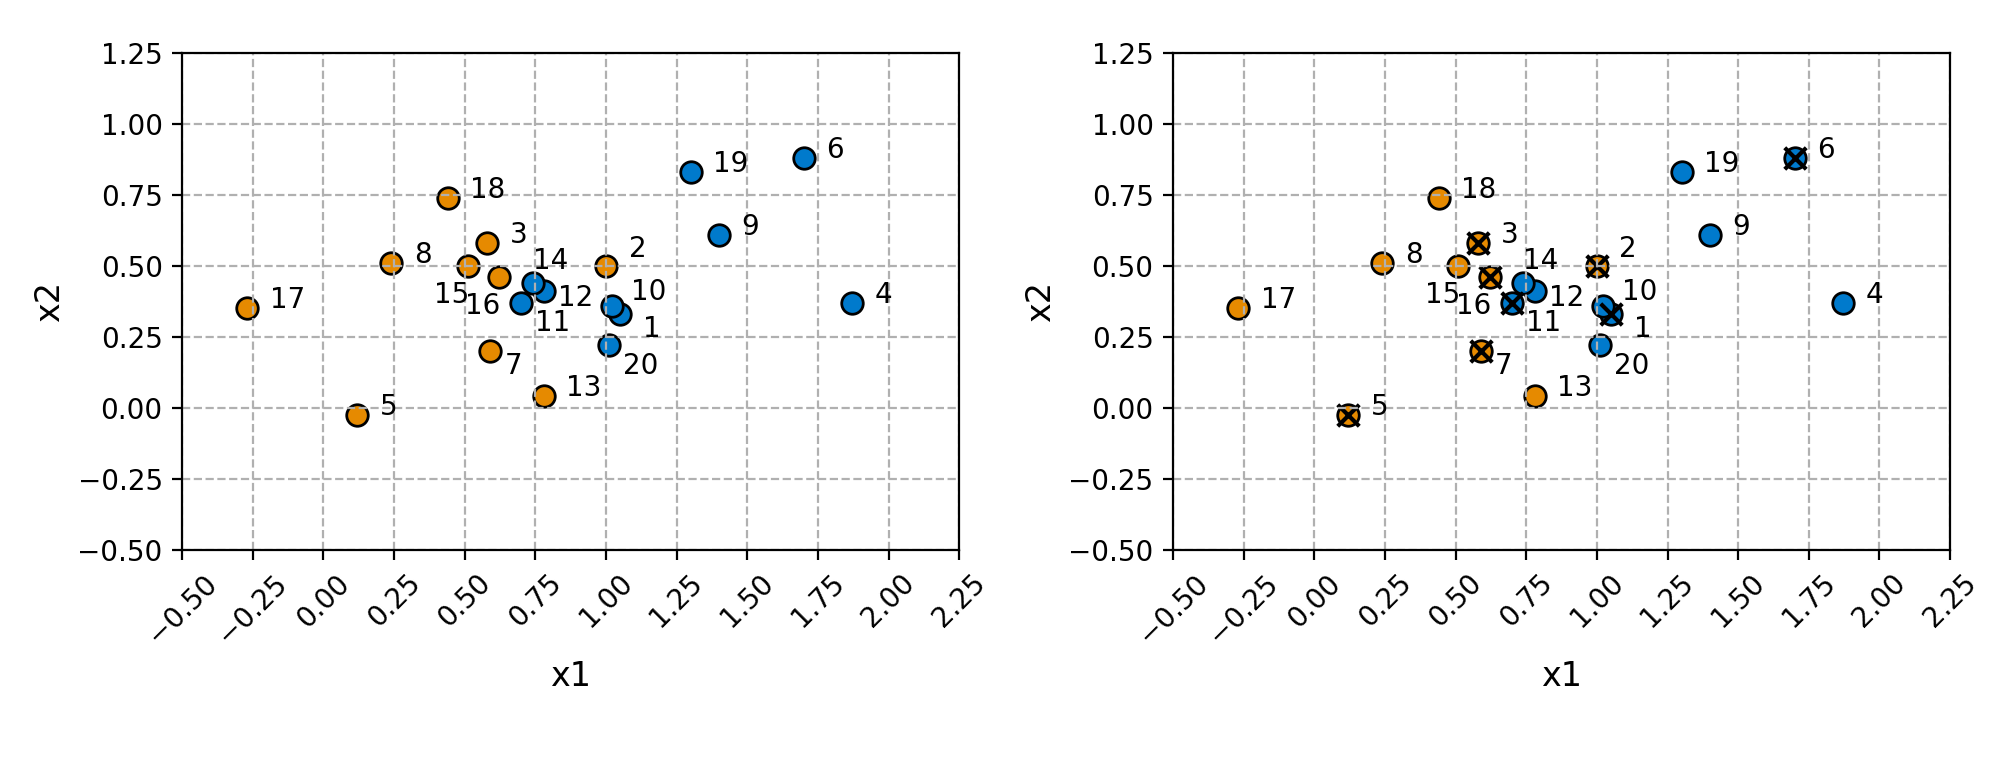
\includegraphics[height = 4.5cm, width =  12cm]{"Part 3 - Learning Systems/Supervised Learning/k-Nearest Neighbors/figures/cnndataset.png"}
    \caption{Examples locations of a hypothetical two class training set $\mathcal{T}$ presented in Table \ref{tab:cnndataset}. On the right, the marked examples represent the chosen examples to form the reference set $S$.}
    \label{fig:cnndataset}
\end{figure}

\subsection{Nearest Neighbor Structural Risk Minimization}

NNSRM \cite{nnsrm:2003}, the CNN, also aims to select examples at the order of the classes, however, NNSRM is not sensitive to the presentation order of the examples in the training set. 

NNSRM finds the most significant training examples such that, for all $\mathbf{x}^{(i)} \in \mathcal{T}$, 1$NN(\mathbf{x}^{(i)}) = y^{(i)}$, i.e., the $R_{emp}$ (empirical risk or training error) is 0. For a two class problem, let $\rho(\mathbf{x}^{(i)},\mathbf{x}^{(j)})$ be the distance between examples $\mathbf{x}^{(i)}$ and $\mathbf{x}^{(j)}$ so that $y^{(i)} = -1$ and $y^{(j)} = 1$. Let $d_k$ be an ascendant ordered list of distances computed between each two elements of opposite classes for $k = 1, 2, 3 \: .. \: \#(y=1) * \#(y=-1)$.

Algorithm \ref{alg:nnsrm} depicts the operation of the NNSRM. While $R_{emp} > 0$ the pair of examples from opposite classes must be found and they must be added to $S$ in case they aren't there. These examples must be found based on the increasing order of distances in $d_k$.

\vspace{0.2cm}

\begin{algorithm}[H]
    \caption{Nearest Neighbor with Structural Risk Minimization}
	\label{alg:nnsrm}
        
    Parameters: $\mathcal{T}$
    
    Output: $S$
    
    
    \begin{algorithmic}[1] 
    \STATE $S \gets \emptyset$
   
    \STATE $k \gets 1$ 
   
   \COMMENT{$R_{emp}$ consists in the training error}
   
    \WHILE{$R_{emp} > 0$}
   
    \STATE find ($x_i$,$x_j$) such that $\rho(x_i,x_j) = d_k$ and $y_i \neq y_j$     
    
    \IF{$x_i \notin S$}
            \STATE $S \gets S + (x_i, y_i)$
    \ENDIF
    
    \IF{$x_j \notin S$}
          \STATE $S \gets S + (x_j, y_j)$
    \ENDIF
    \STATE $k = k + 1$     
    
    \ENDWHILE 
    \end{algorithmic}
    
    
\end{algorithm}

\vspace{0.2cm}

Figure \ref{fig:nnsrmdataset} presents the result of the execution of the NNSRM for the training set of Table \ref{tab:cnndataset}. Based on the result, it is possible to notice that the NNSRM, in contrast to CNN, is not sensitive to the presentation order of the training examples. Nonetheless, the algorithm can still be affected by noisy examples. 

\begin{figure}[ht!]
    \centering
    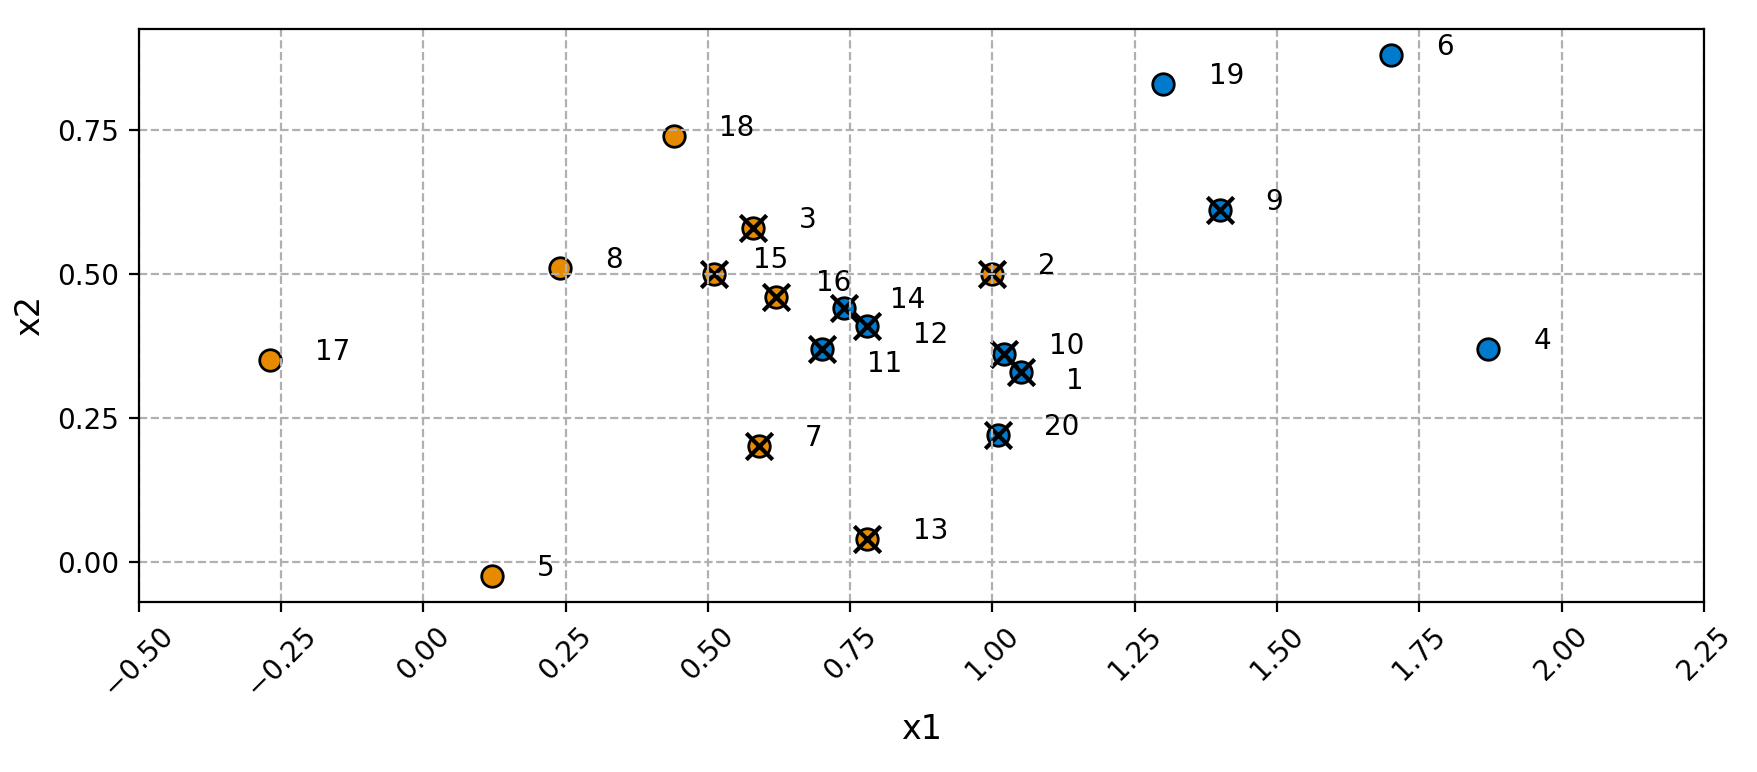
\includegraphics[height = 4.5cm, width =  10cm]{"Part 3 - Learning Systems/Supervised Learning/k-Nearest Neighbors/figures/nnsrmdataset.png"}
    \caption{Training examples locations of a hypothetical two class training set $\mathcal{T}$ and the examples selected by the NNSRM.}
    \label{fig:nnsrmdataset}
\end{figure}

\section{Strengths, Weaknesses and Applications of \textit{k}NN}

Despite its simplicity, the canonical \textit{k}NN has several advantages that make it suitable for many domains. In contrast, some characteristics of the method may represent weaknesses for some other domains. 
\vspace{0.2cm}

\noindent Among the \textit{k}NN strengths are:

\begin{itemize}
    \item Simple and intuitive: the training phase consists solely in the storage of the training set in the computer memory. The test phase, basically, consists in computing the distance from each training example to the test example;
    \item In the case of a proper training set, the \textit{k}NN is comparable to other state-of-art methods in terms of predictive performance;
    \item The method does not rely on any statistical assumption of the problem, i.e., it is nonparametric; and
    \item Easy control of noise robustness via parameter $k$.
\end{itemize}

\noindent Among the \textit{k}NN weaknesses are:


\begin{itemize}
    \item Its computational cost for the test phase is acknowledged as one of main disadvantages;  
    \item Setting a proper value to $k$ is not an intuitive task; and
    \item For large datasets, as well as the computational cost, the memory requirements for storing the dataset may make prohibitive its use. 
    
\end{itemize}

The \textit{k}NN and its variations are general purpose methods and may, virtually, be applied to any problem domain suach as: road traffic prediction \cite{XU2020104}; image recognition \cite{CHEN201878}; software defect prediction \cite{GOYAL201415}; voice recognition \cite{CHEN2021932.e1}; etc.

\section{Exercises}

All resources necessary for the exact reproduction of the experiments in the exercises below are provided in a python notebook available at: \url{https://colab.research.google.com/drive/1vzQMXbRJAyrqE7T54G-r0o8TD1bQA1Cs?usp=sharing} 

\vspace{0.2cm}

Notice that a basic knowledge about Python language and libraries such as Pandas and Matplotlib is essential.

\vspace{0.2cm}

\noindent \textbf{Question 1:}  Given the training and testing datasets depicted in Figure \ref{fig:ex1datasets}, implement and compute the overall accuracy for the canonical \textit{k}NN for $k \in \{1, 3, 5, 7, 9\}$. 

\begin{figure}
\centering
\begin{subfigure}[b]{0.5\textwidth}
  \centering
  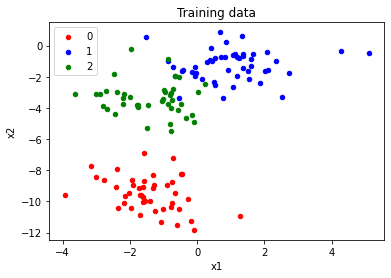
\includegraphics[width=\textwidth]{ "Part 3 - Learning Systems/Supervised Learning/k-Nearest Neighbors/figures/ex1_train.png"}
\end{subfigure}%
\begin{subfigure}[b]{0.5\textwidth}
  \centering
  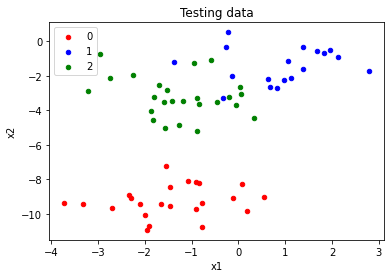
\includegraphics[width=\textwidth]{ "Part 3 - Learning Systems/Supervised Learning/k-Nearest Neighbors/figures/ex1_test.png"}
\end{subfigure}
\caption{Training (left) and test (right) examples for the exercises.}
\label{fig:ex1datasets}
\end{figure}

\vspace{0.2cm}

\noindent \textbf{Question 2:} Respecting the order of the training dataset already defined, implement and perform the CNN algorithm and: (i) show the resulting $S$ subset and (ii) the accuracy for a \textit{k}NN so that $k \in \{1, 3\}$.

\vspace{0.2cm}

\noindent \textbf{Question 3:} Considering the training dataset presented in Table \ref{tab:cnndataset}, implement the two class NNSRM algorithm and plot the resulting subset.

\bibliographystyle{unsrt}
\bibliography{bibliography}
